\section{Symmetries and Interactions}%
\label{sec:theo_symmetries_interactions}

The SM is a relativistic quantum field theory which describes particles and
their interaction using space-time dependent fields $\phi_i(\myvec{x})$. The
field dynamics are determined by the \emph{Lagrangian density} $\lagrange$,
which is a function of the fields $\phi_i$ and their space-time derivatives
$\partial_\mu \phi_i = \partial \phi_i / \partial x^\mu$ ($\mu = 0, 1, 2,
3$). The evolution of the fields in time follows from the principle of
stationary action, i.e.\ by extremising the action
$S = \int \mathrm{d}^4x \, \lagrange(\phi_i, \partial_\mu \phi_i)$, which yields
the Euler--Lagrange equations
\begin{align*}
  \partial_{\mu} \left( \frac{\partial \lagrange}{\partial (\partial_{\mu} \phi_i)} \right) - \frac{\partial \lagrange}{\partial \phi_i} = 0 \,\text{.}
\end{align*}
For a given Lagrangian, the Euler--Lagrange equations provide the ``equations of
motion'' of the fields. The Lagrangian density is hereafter simply referred to
as the \emph{Lagrangian}.

A continuous transformation of the fields that leaves the Lagrangian unchanged
is referred to as a \emph{gauge transformation}. The fields resulting from this
transformation follow the same equations of motion and therefore describe the
same physical system. This invariance is referred to as \emph{gauge invariance}
or \emph{gauge symmetry}.
% An external observer cannot distinguish between fields related by gauge
% transformations and therefore the symmetry is considered an \emph{internal
% symmetry} of the theory.
Continuous symmetries of the Lagrangian are characterised by Lie groups, the
most important ones for the description of the SM being the unitary group
$U(1)$, and the special unitary groups $SU(2)$ and $SU(3)$. Any element of a
unitary group can be written as
\begin{align*}
  \hat{U} = \exp\big[ i \theta_a G^a \big] \,\text{,}
\end{align*}
where $\theta_a$ are real parameters, and $G^a$ are the generators of the group.
% , and summation over repeated indices is implied.
A Lagrangian that is invariant to a transformation $\hat{U}$ of the fields with
parameters $\theta_a$ is said to possess \emph{global} gauge invariance. The
more restrictive case where the Lagrangian is invariant with respect to
transformations of the fields with space-time dependent parameters
$\theta_a(\myvec{x})$ is referred to as \emph{local} gauge invariance.

This is illustrated in the case of the Lagrangian of the Dirac field of mass $m$
given by
\begin{align}
  \lagrange_{\text{Dirac}} = \bar{\psi} (i \gamma^\mu  \partial_\mu - m) \psi \,\text{,}
  \label{eq:dirac_lagrangian}
\end{align}
where $\psi$ ($\bar{\psi} = \psi^\dagger \gamma^0$) are (adjoint) Dirac spinors,
and $\gamma^\mu$ are the Dirac matrices. \Cref{eq:dirac_lagrangian} possesses
global gauge invariance with respect to $U(1)$ transformations given by
$\psi \to \psi^\prime = \exp[ i q \theta ] \psi$, where $q$ is an arbitrary
constant (for the moment). However, when performing a local transformation by
letting the parameter be a function of space-time, i.e.\
$\theta \to \theta(\myvec{x})$, the invariance of the Lagrangian is spoiled due
to the derivative acting on the space-time dependent phase factor. One might
impose $U(1)$ local gauge invariance on the Lagrangian by adding terms to
\Cref{eq:dirac_lagrangian} that cancel the additional
contributions. Conventionally, this is done by substituting the derivative
$\partial_\mu$ by a gauge covariant derivative $D_\mu$ that transforms as
$D_\mu\psi \to \exp[ i q \theta(\myvec{x}) ] D_\mu\psi$, thus recovering local
gauge invariance. A definition of $D_\mu$ with these properties requires the
introduction of a new massless vector field, referred to as a \emph{gauge
  field}, with appropriate transformation properties:
\begin{align}
  D_\mu = \partial_\mu + i q A_\mu \qquad \text{with} \qquad A_\mu \xrightarrow{U(1)} A_\mu^\prime = A_\mu - \partial_\mu \theta(\myvec{x}) \,\text{.}
  \label{eq:covariant_derivative_qed}
\end{align}
The additional term introduced by substituting $\partial_\mu \to D_\mu$ in
\Cref{eq:dirac_lagrangian} is interpreted as an interaction between fermions and
vector bosons of the gauge field.

The principle of local gauge invariance can be used to obtain the Lagrangian of
quantum electrodynamics (QED) describing electromagnetic interactions. The
symmetry group of QED is $U(1)_{Q}$, the subscript $Q$ indicating that the
generator of the group is the electric charge operator. Imposing local gauge
invariance by substituting \Cref{eq:covariant_derivative_qed} into the Dirac
Lagrangian yields the interaction term
\begin{align*}
  \lagrange_{\text{int.}} = - q \bar{\psi} \gamma^\mu \psi A_\mu \,\text{.}
\end{align*}
In the case of QED, the field $A^\mu$ is identified as the four-potential of the
electromagnetic field, and $q$ as the electric charge of the fermion.
% The interaction term that was included to perserve local gauge invariance corresponds
Thus, the interaction term describes the coupling between photons and fermions
with electric charge $q$. For a single type of fermion, the Lagrangian of QED is
given by
\begin{align*}
  \lagrange_{\text{QED}} = \underbrace{\lagrange_{\text{Dirac}}}_{\text{Free fermion field}}
  \hspace*{1em}
  \underbrace{- q \bar{\psi} \gamma^\mu \psi A_\mu}_{\text{Fermion--photon interaction}}
  \hspace*{1em}
  \underbrace{- \frac{1}{4} F_{\mu\nu} F^{\mu\nu}}_{\text{Photon field kinetic term}} \,\text{,}
\end{align*}
which additionally includes the Lagrangian of the free photon field, referred to
as the \emph{kinetic term} of the field, defined by the electromagnetic tensor
$F_{\mu\nu} = \partial_\mu A_\nu - \partial_\nu A_\mu$. This additional term
also fulfils the local gauge invariance with respect to $U(1)_Q$.

The principle of local gauge invariance is at the heart of the SM where it is
used to great success in describing the three fundamental interactions. The
symmetry group of the SM is
\begin{align*}
  SU(3)_{\text{colour}} \otimes SU(2)_{\text{L}} \otimes U(1)_Y \,\text{,}
\end{align*}
where $SU(3)_{\text{colour}}$ is the symmetry of the strong interaction, and
$SU(2)_{\text{L}} \otimes U(1)_Y$ the symmetry of the unified description of the
electromagnetic and weak interaction. These will be introduced in
\Cref{sec:theory_qcd} and \Cref{seq:theory_ewk}, respectively.


\subsection{Quantum Chromodynamics}%
\label{sec:theory_qcd}

Quantum chromodynamics (QCD) is the theory describing the interactions of quarks
and gluons. The fundamental charge of QCD is colour charge which comes in three
distinct colours referred to as red, green, and blue (r, g, b). The quark fields
are consequently written in terms of the three component objects
\begin{align*}
  \psi =
  \begin{pmatrix}
    q_\text{r} \\
    q_\text{g} \\
    q_\text{b}
  \end{pmatrix}
  \qquad
  \text{and}
  \qquad
  \bar{\psi} =
  \begin{pmatrix}
    \bar{q}_\text{r} & \bar{q}_\text{g} & \bar{q}_\text{b}
  \end{pmatrix} \,\text{,}
\end{align*}
in which $q_i$ ($\bar{q}_i$) represents the (adjoint) Dirac spinor describing
the quark field with colour $i$. The symmetry group of the strong interaction is
$SU(3)_{\text{colour}}$, the subscript indicating that elements of the group act
in colour-space. The generators of $SU(3)_{\text{colour}}$ are taken to be
\begin{align*}
  T_a = \frac{1}{2} \lambda_a \qquad \text{for} \qquad a = 1, \dots, 8 \,\text{,}
\end{align*}
where $\lambda_a$ are the Gell-Mann matrices.\footnote{Mathematical objects with
  an upper Latin index and those with a lower Latin index are assumed to be
  equivalent.} The theory of QCD is referred to as a Yang--Mills gauge
theory~\cite{Yang:1954ek} since the elements of $SU(3)_{\text{colour}}$ do not
commute in general, i.e.\ the symmetry group is non-Abelian. The commutation
relation between the generators is given by $[T_a, T_b] = i f_{abc} T^c$,
defining the structure constants $f_{abc}$ of the group.

The principle of local gauge invariance with respect to $SU(3)_{\text{colour}}$
is used to obtain the Lagrangian of QCD. Let the local gauge transformation of
the quark fields be
\begin{align*}
  \psi \to \psi^\prime = \exp[ i g_{\text{s}} \theta_a(\myvec{x}) T^a] \psi \,\text{,}
  %\qquad
  %\bar{\psi} \to \bar{\psi}^\prime = \bar{\psi} \exp[ - i g_{\text{s}} \theta_a(\myvec{x}) T^a]  \,\text{,}
\end{align*}
where $g_{\text{s}}$ is referred to as the strong coupling constant. The gauge
covariant derivative is then
\begin{align*}
  D_\mu = \partial_\mu + i g_{\text{s}} G_\mu^a T_a \,\text{,}
  %\qquad \text{with} \qquad
  %G_\mu^k \xrightarrow{SU(3)_{\text{colour}}} {G_\mu^k}^\prime = G_\mu^k  - \partial_\mu \theta^k(\myvec{x}) - g_{\text{s}} {f_{ij}}^k \theta^i(\myvec{x}) G_\mu^j \,\text{,}
\end{align*}
which introduces eight gauge fields $G_\mu^a$ corresponding to the eight gluons
of QCD. To ensure local gauge invariance, the gluon fields have to transform
according to
\begin{align*}
  G_\mu^k \xrightarrow{SU(3)_{\text{colour}}} {G_\mu^k}^\prime = G_\mu^k  - \partial_\mu \theta^k(\myvec{x}) - g_{\text{s}} {f_{ij}}^k \theta^i(\myvec{x}) G_\mu^j \,\text{.}
\end{align*}
Furthermore, the Lagrangian of QCD has to account for the energy density of the
gluon fields (and their interactions). This contribution is given by the kinetic
term of the gluon fields and reads
\begin{align*}
  \lagrange_{g} = - \frac{1}{4} G_{\mu\nu}^{a} G^{\mu\nu}_{a} \,\text{,}
\end{align*}
where $G_{\mu\nu}^a$ are the gluon field strength tensors defined as
\begin{align*}
  G_{\mu\nu}^a = \partial_\mu G_\nu^a - \partial_\nu G_\mu^a - g_{\text{s}} {f^{a}}_{bc} G_\mu^b G_\nu ^c \,\text{.}
\end{align*}
The Lagrangian of QCD for a single flavour of quark with mass $m$ is
consequently given by
\begin{align*}
  \lagrange_{\text{QCD}} =
  \underbrace{\bar{\psi} (i \gamma^\mu \partial_\mu - m) \psi}_{\text{Free quark field}}
  \hspace*{1em}
  \underbrace{- g_{\text{s}} (\bar{\psi} \gamma^\mu T_a \psi) G_\mu^a}_{\text{Quark--gluon interactions}}
  \hspace*{1em}
  \underbrace{- \frac{1}{4} G_{\mu\nu}^a G^{\mu\nu}_a}_{\text{Gluon field kinetic term}} \,\text{.}
  %\label{eq:qcd_lagrangian}
\end{align*}
This Lagrangian describes the free quark field, the interactions of quarks with
the eight gluons, and the kinetic energy of the gluon fields. The non-Abelian
nature of the $SU(3)_{\text{colour}}$ group, meaning a set of indices exists
such that $f_{abc} \neq 0$, gives rise to the distinct structure of QCD through
the kinetic term of the gluon fields. This term includes self-interactions
between gluons which correspond to, in the language of Feynman diagrams, triple
and quartic interaction vertices between gluons. Gluons themselves are carriers
of colour charge which leads to this behaviour. This is unlike the photon of QED
which does not carry electrical charge and thus does not couple to itself.

Two important features of the theory of QCD are highlighted in the following:
\begin{description}

\item[Colour confinement] Due to the dynamics of the gluon self-interactions,
  free quarks or gluons cannot be observed in nature~\cite{Wilson:1974sk}. For
  example, separating the quarks of a quark-antiquark pair leads to the
  formation of \emph{flux tubes} in the gluon field strength that result in a
  linear increase in field energy with separation of the quarks. Eventually, the
  energy stored in the gluon field is sufficiently large to create a
  quark-antiquark pair from the vacuum. This process repeats until only quarks
  or gluons bound into colourless composite particles (colour singlet states)
  remain. The most prevalent bound states of quarks are (anti-)baryons
  consisting of three (anti-)quarks, and mesons consisting of a quark-antiquark
  pair. The $SU(3)_{\text{colour}}$ symmetry also allows for colour singlet
  states of multiple gluons referred to as
  \emph{glueballs}~\cite{Fritzsch:1972jv,Fritzsch:1975tx}, or other combinations
  of quarks such as tetra- ($q_1 \bar{q}_2 q_3 \bar{q}_4$) or pentaquarks
  ($q_1 q_2 q_3 q_4 \bar{q}_5$)~\cite{Gell-Mann:1964ewy}.

\item[Running coupling \& asymptotic freedom] The strong coupling constant,
  frequently expressed as $\alphas = g_{\text{s}}^2 / (4 \pi)$ in analogy to the
  fine-structure constant $\alpha = e^2 / (4 \pi)$ of QED, is not constant but
  varies as a function of the momentum transfer $Q$ of an interaction. A quark
  scattering process involving the exchange of a gluon is represented by an
  infinite number of Feynman diagrams with different higher-order corrections,
  for example diagrams with additional quark or gluon loops. A process referred
  to as \emph{renormalisation} absorbs these corrections into an effective
  coupling constant, the coupling consequently becoming a function of
  $Q^2$. This effect occurs in both QED and QCD, however, with distinct
  signatures. While the coupling $\alpha(Q^2)$ of QED increases with $Q^2$,
  $\alphas(Q^2)$ of QCD decreases with $Q^2$ due to gluon self-interactions. The
  high-$Q^2$ behaviour of \alphas is referred to as \emph{asymptotic
    freedom}~\cite{Gross:1973id,Politzer:1973fx}.
  % At large $Q^2$ the value of \alphas is small such that perturbative methods
  % can be used to obtain cross section predictions.
\end{description}


\subsection{Theory of the Electroweak Interaction}%
\label{seq:theory_ewk}

The principle of local gauge invariance was previously used to obtain the
Lagrangians of QED and QCD. The characteristics of the weak interaction make
this approach more difficult. First, the mediators of the interaction are
massive with masses of ~\cite{pdg2020}
\begin{align*}
  m_W = \SI{80.377 +- 0.012}{\GeV}
  \qquad \text{and} \qquad
  m_{Z} = \SI{91.1876 +- 0.0021}{\GeV} \text{.}
\end{align*}
Second, the symmetry with respect to parity (space-inversion) transformations is
violated~\cite{Wu:1957my}. Lastly, the charged-current weak interaction couples
fermions of different flavour that differ by one unit in electric charge. Due to
these characteristics, the construction of a gauge theory of the weak
interaction that respects local gauge invariance requires the introduction of
new mechanisms.
% that were not needed for the description of QED and QCD.

\subsubsection{Electroweak Unification}

The theory of the electroweak interaction was developed by Glashow, Salam, and
Weinberg in the 1960s to unify the electromagnetic and weak interactions in a
single model~\cite{Glashow:1961tr,Salam:1964ry,Weinberg:1967tq}. The theory is
constructed as a non-Abelian gauge theory based on a symmetry group referred to
as $SU(2)_{\text{L}} \otimes U(1)_{Y}$, the meaning of the subscripts will be
illustrated in the following.

First, a new quantum number referred to as \emph{weak isospin} denoted by $I$,
and its component along the 3-axis, $I_3$, is introduced. The charged-current
weak interaction violates parity symmetry maximally, meaning it only couples to
fermionic fields with left-handed chirality.\footnote{Chirality of a Dirac field
  is defined by the operator
  $\gamma^5 \coloneq i \gamma^0 \gamma^1 \gamma^2 \gamma^3$. The eigenvectors of
  $\gamma^5$ are states of well-defined chirality with eigenvalues of $+1$ or
  $-1$, referred to as right- and left-handed chiral states, respectively. Any
  spinor can be written as a superposition of right- and left-handed chiral
  states using the projection operators
  $P_{\text{R/L}} = (1 \pm \gamma^5) / 2$.} An appropriate weak isospin grouping
of SM fermions is chosen in anticipation of a $SU(2)$ symmetry.
% Based on the experimental observation that the charged-current weak
% interaction only couples to particles (antiparticles) with left-handed
% (right-handed) chirality, an appropriate grouping of the SM fermions is
% chosen.
Left-handed fermion fields are grouped into weak isospin doublets given by
\begin{align*}
  \begin{pmatrix}
    \nu_{e} \\
    e^{-}
  \end{pmatrix}_{\text{L}},
  \begin{pmatrix}
    \nu_{\mu} \\
    \mu^{-}
  \end{pmatrix}_{\text{L}},
  \begin{pmatrix}
    \nu_{\tau} \\
    \tau^{-}
  \end{pmatrix}_{\text{L}}
  \qquad
  \begin{pmatrix}
    u \\
    d
  \end{pmatrix}_{\text{L}},
  \begin{pmatrix}
    c \\
    s
  \end{pmatrix}_{\text{L}},
  \begin{pmatrix}
    t \\
    b
  \end{pmatrix}_{\text{L}}
  \qquad
  \text{with}
  \qquad
  I = \frac{1}{2}, I_3 = \pm \frac{1}{2} \,\text{,}
\end{align*}
where the upper (lower) components correspond to $I_3 = +\frac{1}{2}$
($I_3 = -\frac{1}{2}$), and nine singlet states for right-handed fermion fields
\begin{align*}
  e^{-}_{\text{R}}, \mu^{-}_{\text{R}}, \tau^{-}_{\text{R}},
  u_{\text{R}}, d_{\text{R}}, c_{\text{R}}, s_{\text{R}}, t_{\text{R}}, b_{\text{R}}
  \qquad
  \text{with}
  \qquad
  I = 0, I_3 = 0 \,\text{,}
\end{align*}
where the subscripts L and R refer to the projection of the fields into their
left- and right-handed chiral components,
respectively. % The quark eigenstates of
% the weak interaction are indicated by $d^\prime, s^\prime, b^\prime$ which are
% related to the quark mass eigenstates via the Cabibbo--Kobayashi--Maskawa
% matrix~\cite{Cabibbo:1963yz,Kobayashi:1973fv}.
Right-handed neutrinos are omitted since they are not part of the SM.
% \footnote{The determination of the nature of neutrinos is still an active area
% of physics research. In the SM, neutrinos are assumed to be massless which is
% in disagreement with the observation of neutrino oscillations. Under the
% assumption that neutrinos are Dirac particles, the non-vanishing mass would
% suggest that there is mixing between left- and right-handed chiral states of
% neutrinos. However, in the current theory right-handed neutrinos would be
% ``sterile'' meaning they would not interact via any of the interactions
% described by the SM. Alternative proposals are that neutrinos are not Dirac
% but Majorana particles~\cite{Majorana:1937vz}, which are particles that are
% identical to their antiparticles.}
Given this grouping, $SU(2)_{\text{L}}$ transformations only affect fermion
fields with left-handed chirality, thus motivating the choice of subscript.
% \todo{If we are assuming massless quarks -> mass and weak eigenstates are the
% same.}

Second, a quantum number referred to as the \emph{weak hypercharge} is defined
according to
\begin{align*}
  Y = 2 (Q - I_3) \,\text{,}
\end{align*}
where $Q$ refers to the electric charge. Since the electric charge differs
between the upper and lower component of the $SU(2)_{\text{L}}$ doublets, a
$SU(2)_{\text{L}}$ transformation would violate the $U(1)_Q$ symmetry of
QED. Therefore, the weak hypercharge is defined such that both components of a
$SU(2)_{\text{L}}$ doublet have the same value of $Y$. The broken $U(1)_Q$
symmetry is consequently replaced by a $U(1)_Y$ symmetry, which uses $Y$ as the
generator of the group instead. The $U(1)_Q$ symmetry of QED will later be
recovered in a process referred to as \emph{electroweak symmetry breaking}
(EWSB).

The principle of local gauge invariance with respect to the
$SU(2)_{\text{L}} \otimes U(1)_Y$ group is invoked to generate the interactions
of the electroweak theory. In the following, the weak isospin doublets are
denoted as $\chi_{\text{L}}$ and weak isospin singlets as $\psi_{\text{R}}$. The
gauge transformations with space-time dependent parameters $\alpha_a$
($a = 1, 2, 3$) and $\beta$ transform the fields as follows
\begin{align*}
  &\chi_{\text{L}} \to \chi_{\text{L}}^\prime = \exp\left[ i g \alpha_a(\myvec{x}) \frac{\sigma^a}{2} + i g^\prime \beta(\myvec{x}) \frac{Y}{2} \right] \chi_{\text{L}} \\
  &\psi_{\text{R}} \to \psi_{\text{R}}^\prime = \exp\left[ i g^\prime \beta(\myvec{x}) \frac{Y}{2} \right] \psi_{\text{R}} \,\text{,}
\end{align*}
where $g$ and $g^\prime$ are coupling constants, and $\sigma^a$ are the Pauli
matrices. The gauge covariant derivative is given by
\begin{align*}
  D_\mu = \partial_\mu
  + i g W^a_\mu \frac{\sigma_a}{2}
  + i g^\prime B_\mu \frac{Y}{2} \,\text{,}
\end{align*}
where it is implied that the Pauli matrices only act on $\chi_{\text{L}}$ and
not on $\psi_{\text{R}}$. Four gauge fields, $W_\mu^a$ ($a = 1, 2, 3$) and
$B_\mu$, associated with the $SU(2)_{\text{L}}$ and $U(1)_Y$ symmetry are
introduced. These fields transform, in analogy to QED and QCD, as follows
\begin{align*}
  W_\mu^k &\xrightarrow{SU(2)_{\text{L}} \otimes SU(1)_Y} {W_\mu^k}^\prime = W_\mu^k - \partial_\mu \alpha^{k}(\myvec{x}) - g {f_{ij}}^k \alpha^{i} W_\mu^j \\
  B_\mu   &\xrightarrow{SU(2)_{\text{L}} \otimes SU(1)_Y} {B_\mu}^\prime = B_\mu - \partial_\mu \beta(\myvec{x}) \,\text{,}
\end{align*}
where $f_{ijk}$ are the structure constants of $SU(2)_{\text{L}}$ with the
generators of the group taken to be $\frac{1}{2} \sigma_a$.  Substituting the
gauge covariant derivative into the kinetic term of the Dirac Lagrangian yields
the interaction terms of the electroweak theory for left- and right-handed
chiral fields
\begin{align}
  &\lagrange_{\text{int.}}^{\text{L}} = i \bar{\chi}_{\text{L}} \gamma^\mu \left[i g W_\mu^a \frac{\sigma_a}{2} + i g^\prime B_\mu \frac{Y}{2} \right] \chi_{\text{L}} \label{eq:theory_electroweak_left} \\
  &\lagrange_{\text{int.}}^{\text{R}} = i \bar{\psi}_{\text{R}} \gamma^\mu \left[i g^\prime B_\mu \frac{Y}{2} \right] \psi_{\text{R}} \,\text{.} \label{eq:theory_electroweak_right}
\end{align}
The four fields occurring in the interaction terms do not represent the physical
fields observed in nature. Given the choice of Pauli matrices as the generators
of $SU(2)_{\text{L}}$, the fields $W_\mu^1$ and $W_\mu^2$ are associated with
charged-current interactions, and $W_\mu^3$ and $B_\mu$ with neutral-current
interactions. The physical fields of the charged-current interaction can be
identified as
\begin{align*}
  W_\mu^\pm = \frac{1}{\sqrt{2}} (W_\mu^1 \mp i W_\mu^2) \,\text{.}
\end{align*}
% in analogy to the weak isospin ladder operators.
Furthermore, the physical fields describing the neutral-current interactions via
the exchange of $Z$ bosons and photons can be expressed as a linear combination
of the $W_\mu^3$ and $B_\mu$ gauge fields. Experimental results show that the
$Z$ boson couples to both left- and right-handed chiral states, although not
equally, and therefore such a mixing is required. The mixing can be described by
a rotation of the fields by the weak mixing angle $\theta_{\text{W}}$ according
to
\begin{align*}
  \begin{pmatrix}
    A_\mu \\
    Z_\mu
  \end{pmatrix}
  =
  \begin{pmatrix}
    \cos\theta_{\text{W}} & \sin\theta_{\text{W}} \\
    -\sin\theta_{\text{W}} & \cos\theta_{\text{W}}
  \end{pmatrix}
  \begin{pmatrix}
    B_\mu \\
    W_\mu^3
  \end{pmatrix} \,\text{.}
\end{align*}
The weak mixing angle must be chosen such that
\Cref{eq:theory_electroweak_left,eq:theory_electroweak_right} reproduce the
coupling of QED, namely the photon must couple equally to left- and right-handed
particles with a coupling constant $e$. This yields the condition
\begin{align*}
  e = g \sin\theta_{\text{W}} = g^\prime \cos\theta_{\text{W}} \,\text{,}
\end{align*}
% \todo{Note ways to express sin / cos as a function of $g$ and $g^\prime$.}
connecting the QED coupling constant with the coupling constants $g$ and
$g^\prime$ of the electroweak interaction. Finally, the kinetic term of the
$W_\mu^a$ and $B_\mu$ fields is given, in analogy to QED and QCD, by
\begin{align*}
  \lagrange_{W, Z, \gamma} =
  - \frac{1}{4} W_{\mu\nu}^a W^{\mu\nu}_a
  - \frac{1}{4} B_{\mu\nu} B^{\mu\nu} \,\text{,}
\end{align*}
where the field strength tensors are defined as
\begin{align*}
  W_{\mu\nu}^a &= \partial_\mu W_\nu^a - \partial_\nu W_\mu^a - g {f^a}_{bc} W_\mu^b W_\nu^c \\
  B_{\mu\nu} &= \partial_\mu B_\nu - \partial_\nu B_\mu \,\text{.}
\end{align*}
Since $SU(2)_{\text{L}}$ is a non-Abelian group, triple and quartic gauge boson
couplings are introduced through the kinetic term of the $W_\mu^a$ fields.


\subsubsection{The Brout--Englert--Higgs Mechanism}

In the context of the electroweak theory, the non-zero masses of the gauge
bosons (and fermions) have been ignored thus far. Inserting gauge field mass
terms into the Lagrangian, for example for the physical $Z_\mu$ field with mass
$m_Z$ according to
\begin{align*}
  \lagrange_{\text{mass}}^{Z} = \frac{1}{2} m_{Z}^2 Z_\mu Z^\mu \,\text{,}
\end{align*}
would violate $SU(2)_{\text{L}} \otimes U(1)_Y$ symmetry due to the
transformation properties of the fields. A mechanism to dynamically generate the
required mass terms was introduced into the electroweak theory by
Weinberg~\cite{Weinberg:1967tq} to address this issue. This mechanism traces
back to Brout, Englert, and Higgs~\cite{Englert:1964et,Higgs:1964pj} and is thus
referred to as the Brout--Englert--Higgs (BEH) mechanism.

The BEH mechanism introduces two complex scalar fields, one electrically charged
and one neutral field, arranged in a weak isospin doublet with $Y = 1$ according
to
\begin{align*}
  \phi =
  \begin{pmatrix}
    \phi^+ \\
    \phi^0
  \end{pmatrix}
  = \frac{1}{\sqrt{2}}
  \begin{pmatrix}
    \phi_1 + i \phi_2 \\
    \phi_3 + i \phi_4
  \end{pmatrix} \,\text{,}
\end{align*}
which can analogously be expressed as four real scalar fields $\phi_i$. The
Lagrangian of the complex scalar fields is given by the Klein--Gordon equation
\begin{align*}
  \lagrange = (\partial_\mu \phi)^\dagger (\partial^\mu \phi) - V(\phi)
\end{align*}
with the potential term denoted by $V(\phi)$. The aim of the BEH mechanism is to
embed the doublet of complex scalar fields into the electroweak theory with a
$SU(2)_{\text{L}}\otimes U(1)_Y$ symmetry. To fulfil the gauge invariance of the
electroweak theory, the potential term can only depend on $\phi^\dagger
\phi$. One such choice is
\begin{align}
  V(\phi) = \mu^2 \phi^\dagger \phi + \lambda (\phi^\dagger \phi)^2
  \label{eq:higgs_potential}
\end{align}
with $\mu^2$ and $\lambda$ being parameters of the potential.\footnote{In terms
  of the renormalisability of the theory, the largest allowed power of
  $\phi^\dagger \phi$ in the Lagrangian is two. See for example
  Ref.~\cite{Peskin:1995ev}.} The potential must be bound from below to have a
well-defined state of minimum potential energy (vacuum state) and therefore
$\lambda$ must be positive. No such restrictions exist for $\mu^2$, leaving two
options. If $\mu^2 > 0$, the vacuum state is $\phi = \myvec{0}$ and $\mu$ is
related to the mass of the scalar field. If $\mu^2 < 0$, the field configuration
$\phi = \myvec{0}$ is at an unstable point and the true vacuum is given by the
condition
\begin{align*}
  \sum_{i = 1}^4 \phi_i^2 = -\frac{\mu^2}{\lambda} \eqqcolon \varv^2 \,\text{,}
\end{align*}
which represents a continuum of degenerate states at a radius of $\varv$ from the
origin in the space spanned by the four real scalar fields. The quantity $\varv$ is
therefore referred to as the \emph{vacuum expectation value} (VEV). Hereafter,
this particular choice of potential is referred to as the Higgs potential. This
choice is illustrated in \Cref{fig:mexican_hat} for a simplified model with only
a single complex scalar field.

\begin{figure}[htbp]
  \centering

  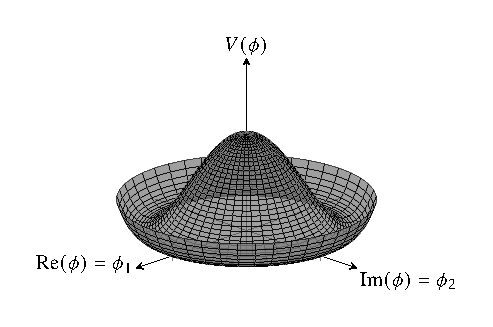
\includegraphics[scale=1.1]{theory/potential}

  \caption[The ``Mexican-hat potential'' of a complex scalar field.]{The
    ``Mexican-hat potential'' of a single complex scalar field as a low
    dimensional example to illustrate the choice of the Higgs potential in the
    SM. The degenerate vacuum states lie in a circle with radius $\varv$ given
    by the condition $\phi_1^2 + \phi_2^2 = \varv^2$. The figure is adapted from
    Ref.~\cite{higgs_potential_tikz}.}%
  \label{fig:mexican_hat}
\end{figure}

The fields $\phi_i$ will assume a configuration that minimises the potential
energy, hence realising one of the infinite number of vacuum states. While the
full Lagrangian still possesses a $SU(2)_{\text{L}} \otimes U(1)_Y$ symmetry,
the spontaneous choice of a vacuum state with non-vanishing VEV appears to break
the symmetry, a process referred to as \emph{spontaneous symmetry
  breaking}. Perturbative methods are used to find solutions to the field
equations of motion, hence the fields have to be expressed as small
perturbations relative to the vacuum state. Let the vacuum state be
\begin{align*}
  \phi_{\text{v}} = \frac{1}{\sqrt{2}}
  \begin{pmatrix}
    0 \\
    \varv
  \end{pmatrix} \,\text{,}
\end{align*}
chosen such that only the neutral component is non-vanishing to ensure that the
$U(1)_Q$ symmetry of QED is recovered after spontaneous symmetry
breaking.\footnote{An infinitesimal $U(1)_Q$ transformation yields
  $(1 + i \epsilon Q) \phi_{\text{v}} = \phi_{\text{v}}$, thus leaving the
  vacuum state unchanged. This is not the case when replacing $Q$ with the
  generators of $SU(2)_{\text{L}}$ or $U(1)_Y$.} Four degrees of freedom for
perturbations relative to the chosen vacuum state exist. Three degrees of
freedom are chosen such that they leave $\phi^\dagger \phi$, and thus $V(\phi)$,
invariant. The remaining degree of freedom alters the value of
$\phi^\dagger \phi$ and therefore $V(\phi)$.\footnote{In the toy model depicted
  in \Cref{fig:mexican_hat}, the degrees of freedom correspond to perturbations
  of the vacuum state in angular and radial direction, respectively.} In the
Lagrangian describing the fields $\phi$, these perturbations appear as three
massless scalar fields and one massive scalar field. The quanta of the massless
fields are referred to as Nambu--Goldstone
bosons~\cite{Nambu:1960tm,Goldstone:1961eq}, however, a suitable gauge
transformation, referred to as the \emph{unitary gauge}, allows to remove the
massless scalar fields from the theory. In unitary gauge, the doublet of complex
scalar fields can be expressed as
\begin{align}
  \phi(\myvec{x}) = \frac{1}{\sqrt{2}}
  \begin{pmatrix}
    0 \\
    \varv + H(\myvec{x})
  \end{pmatrix}
  \label{eq:vacuum_state_perturb}
\end{align}
with $H(\myvec{x}) \in \mathbb{R}$.

% Check: https://arxiv.org/pdf/1704.02311.pdf
Expressing the Higgs potential of \Cref{eq:higgs_potential} in terms of
perturbations of the vacuum state, i.e.\ using \Cref{eq:vacuum_state_perturb},
and dropping terms not depending on $H$ yields
\begin{align}
  V(H) =
  \lambda \varv^2 H^2
  + \lambda \varv H^3
  + \frac{\lambda}{4} H^4 \,\text{.}
  \label{eq:beh_potential}
\end{align}
The first term of $V(H)$ represents the mass term of the scalar field $H$ with a
mass of $m_H = \sqrt{2\lambda} \varv$. The quantum of the scalar field is
referred to as the Higgs boson ($H$).\footnote{Depending on the context, $H$
  refers to the Higgs boson or the scalar field that describes the Higgs field
  in unitary gauge.} The terms cubic and quartic in the scalar field represent
self-interactions between Higgs bosons with coupling strengths defined
as\footnote{There exists no consensus regarding the definition of
  $\lambda_{HHH}$ and $\lambda_{HHHH}$. In this thesis a convention is adopted
  such that the Higgs potential can be expressed as
  \begin{align*}
    V(H) = \frac{m_{H}^2}{2} H^2 + \frac{\lambda_{HHH}}{3!} H^3 + \frac{\lambda_{HHHH}}{4!}
    H^4 \,\text{.}
  \end{align*}
}
\begin{align*}
  \lambda_{HHH} \coloneqq \frac{3 m_{H}^2}{\varv} \qquad \text{and} \qquad \lambda_{HHHH} \coloneqq \frac{3 m_{H}^2}{\varv^2} \,\text{.}
\end{align*}
The Feynman vertices of Higgs boson self-interactions are depicted in
\Cref{fig:vertex_hhh,fig:vertex_hhhh}.

The term of the Klein--Gordon equation involving the space-time derivatives
yield after substituting the $SU(2)_{\text{L}} \otimes U(1)_Y$ gauge covariant
derivative and inserting the physical fields describing the $W$ and $Z$ bosons
\begin{align}
  (D_\mu \phi)^\dagger (D^\mu \phi) =
  \frac{1}{2} (\partial_\mu H) (\partial^\mu H)
  + \left[
  \frac{g^2 \varv^2}{4} W^{-}_\mu {W^{+}}^\mu
  +
  \frac{(g^2 + {g^\prime}^2) \varv^2}{8} Z_\mu Z^\mu
  \right] \left( 1 + \frac{1}{\varv} H \right)^2 \,\text{.}
  \label{eq:higgs_covariant_derivative}
\end{align}
The first term of \Cref{eq:higgs_covariant_derivative} yields the kinetic term
for the scalar field $H$. Moreover, the BEH mechanism dynamically generates mass
terms for the $W^\pm$ and $Z$ bosons while leaving the photon massless. Using
the four parameters of the electroweak theory ($g$, $g^\prime$, $m_{H}$, $\varv$)
the masses of the bosons can be obtained from the Lagrangian such that
\begin{align*}
  &m_W = \frac{1}{2} g \varv  &&m_Z = \frac{1}{2} \sqrt{g^2 + {g^\prime}^2} \, \varv && m_{\text{photon}} = 0 \,\text{.}
\end{align*}
\Cref{eq:higgs_covariant_derivative} additionally describes interaction vertices
of the form $WWH$, $ZZH$, $WWHH$, and $ZZHH$, which are depicted in
\Cref{fig:higgs_vertices}.

\begin{figure}[htbp]
  \centering

  \begin{subfigure}{0.33\textwidth}
    \centering
    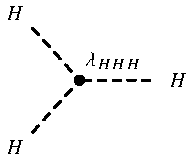
\includegraphics[scale=0.9]{feynman_graphs/higgs_hhh}
    \subcaption{}
    \label{fig:vertex_hhh}
  \end{subfigure}%
  \begin{subfigure}{0.33\textwidth}
    \centering
    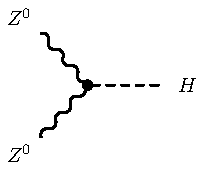
\includegraphics[scale=0.9]{feynman_graphs/higgs_hzz}
    \subcaption{}
  \end{subfigure}%
  \begin{subfigure}{0.33\textwidth}
    \centering
    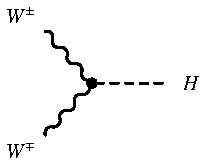
\includegraphics[scale=0.9]{feynman_graphs/higgs_hww}
    \subcaption{}
  \end{subfigure}

  \vspace{1em}

  \begin{subfigure}{0.33\textwidth}
    \centering
    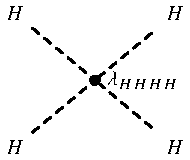
\includegraphics[scale=0.9]{feynman_graphs/higgs_hhhh}
    \subcaption{}
    \label{fig:vertex_hhhh}
  \end{subfigure}%
  \begin{subfigure}{0.33\textwidth}
    \centering
    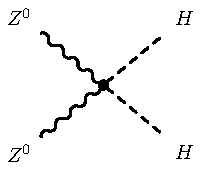
\includegraphics[scale=0.9]{feynman_graphs/higgs_hhzz}
    \subcaption{}
  \end{subfigure}%
  \begin{subfigure}{0.33\textwidth}
    \centering
    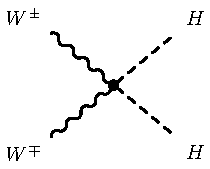
\includegraphics[scale=0.9]{feynman_graphs/higgs_hhww}
    \subcaption{}
  \end{subfigure}

  \caption[Interaction vertices between Higgs, $W$, and $Z$~bosons predicted by
  the SM.]{Interaction vertices between Higgs, $W$, and $Z$~bosons predicted by
    the SM.}%
  \label{fig:higgs_vertices}
\end{figure}

% Prior to the discovery of the Higgs boson, of the four parameters describing
% the electroweak theory the only one left to be determined was the mass of the
% Higgs boson, $m_{H}$. After the discovery of the Higgs boson and the
% measurement of its mass, no unknown parameters remain in the electroweak
% theory.

% Conventionally, the couplings of the electroweak unification are given in terms
% of $e$ and $\sin^2\theta_{\text{W}} = \num{0.23124 +- 0.00004}$ at
% $Q^2 = m_{Z}^2$~\cite{pdg2020}.


\subsubsection{Fermion Masses}

The inclusion of fermion mass terms of the form
\begin{align*}
  \lagrange_{\text{mass}}^{\text{fermion}} = - m \bar{\psi} \psi = - m [ \bar{\psi}_\text{R} \psi_\text{L} + \bar{\psi}_\text{L} \psi_\text{R} ]
\end{align*}
into the Lagrangian violates the gauge invariance with respect to the
$SU(2)_{\text{L}} \otimes U(1)_Y$ symmetry, since fermions with left- and
right-handed chirality transform differently. Instead, fermion mass terms are
generated dynamically through EWSB by introducing interactions between the
fermion fields and the scalar Higgs field, which are referred to as Yukawa
interactions~\cite{Yukawa:1935xg}.

First, the conjugate of the Higgs field $\phi$ is defined as
$\phi^{\text{c}} = i \sigma_2 \phi^*$, such that after after EWSB in unitary
gauge
\begin{align*}
  \phi^{\text{c}} = \frac{1}{\sqrt{2}}
  \begin{pmatrix}
    \varv + H(\myvec{x}) \\
    0
  \end{pmatrix} \,\text{.}
\end{align*}
A Lagrangian of the Yukawa interactions with $SU(2)_{\text{L}} \otimes U(1)_Y$
gauge invariance is defined, here exemplary for the first generation of
fermions, as
\begin{align}
  \lagrange_{\text{Yukawa}} =
  - y_e \bar{L} \phi e_{\text{R}}
  - y_u \bar{Q} \phi^{\text{c}} u_{\text{R}}
  - y_d \bar{Q} \phi d_{\text{R}}
  + \text{h.c.} \,\text{,}
  \label{eq:lagrangian_yukawa}
\end{align}
where $\bar{L}$ and $\bar{Q}$ are the $SU(2)_{\text{L}}$ doublets of the first
generation of leptons and quarks, respectively. The $SU(2)_{\text{L}}$ singlets
for electrons, up-, and down-quarks are denoted as $e_{\text{R}}$,
$u_{\text{R}}$, and $d_{\text{R}}$. Moreover, the coupling constants of the
Yukawa interactions, which are free parameters of the theory, are given by
$y_e$, $y_u$, and $y_d$. Finally, $\text{h.c.}$ represents the hermitian
conjugate of the preceding terms. After EWSB and in unitary gauge
\Cref{eq:lagrangian_yukawa} reads
\begin{align*}
  \lagrange_{\text{Yukawa}} \xrightarrow{\text{EWSB}} \sum_{f \in \{e, u, d\}} -\frac{y_{\hspace{-0.1em}f} \varv}{\sqrt{2}} [ \bar{f}_{\text{L}} f_{\text{R}} + \bar{f}_{\text{R}} f_{\text{L}} ] \left( 1 + \frac{1}{\varv} H \right)
\end{align*}
yielding fermion mass terms with masses
\begin{align*}
  m_{f} = \frac{y_{\hspace{-0.1em}f} \varv}{\sqrt{2}} \,\text{,}
\end{align*}
which are proportional to the Yukawa coupling constants, as well as interactions
between Higgs bosons and fermions with a coupling strength proportional to the
mass of the fermion given by
\begin{align*}
  g_{H\!f\!f} = \frac{m_f}{\varv} \,\text{.}
\end{align*}

The Lagrangian of \Cref{eq:lagrangian_yukawa} can be further generalised to
include the remaining fermion generations, and mixing between the weak and mass
eigenstates of quarks as described by the Cabibbo--Kobayashi--Maskawa
matrix~\cite{Cabibbo:1963yz,Kobayashi:1973fv}.


%%% Local Variables:
%%% mode: latex
%%% TeX-master: "../../phd_thesis"
%%% End:
